\pdfminorversion=7
\documentclass[../main.tex]{subfiles}

\begin{document}
\ifx\chapincluded\undefined
  \begin{refsection}[main-bib]
 \fi

\chapter{Background}
\label{chap:background}
In this chapter, we introduce the contextual background that surrounds
this thesis. In particular, we focus on microarchitectural
optimizations specifically targeting datacenter workloads and we give
an in-depth introduction to serverless computing, what makes it unique
and the challenges surrounding the execution of serverless functions

%Paper giving background on serverless computing \cite{van2018serverless}

% \subsection{Designing a Microarchitecture for the Datacenter}

\section{Serverless Computing}
\label{sec:serverless}

%Communication problem -> what people have done

Over the past couple of decades, cloud computing has revolutionized
the way computing is performed. Traditionally, developers were in
charge of manually provisioning the computing resources that they
needed ahead of time. Another consequence of the traditional model for
managing computing resources is that practitioners needed to consider
how to handle peak application demand. Scaling an entire hosting
infrastructure only to meet peak demand would lead to massive amounts
of wasted resources. On the other hand, not meeting peak demand leads
to unacceptably poor application performance when it is needed the
most. Furthermore, features such as distributing an application across
diverse geographical locations were out of reach of all but the
largest companies. The foundations of cloud computing began to be
publicly known when Google began publishing papers about their
internal architecture around
2003~\cite{qian2009cloud,gfs,dean2008mapreduce,barroso03_web_searc_planet}. These
papers outlined the technological underpinnings of a large-scale
elastic cloud computing service powered by a large aggregation of
commodity computing hardware.

Since Amazon released the first publicly available cloud offering,
\liningfigures{EC2}, in 2006~\cite{qian2009cloud} the popularity of
the cloud has exploded and a plethora of products have been released
to meet practicioners' desire for flexible, infinitely scalable
maintenance-free and cost-effective computing. Following this trend,
serverless computing is a recent addition to the cloud computing
landscape that is quickly gaining popularity. Serverless computing
promises developers quick and easy application deployment without
having to consider how the application is hosted. Serverless is
somewhat of a misnomer since applications developed using this model
are still executed on a server. The name refers to the fact that the
developer is not in charge of deploying the application on a server,
they simply provide the application code and from there they leave it
up the provider to decide how the code is executed. The programming
model underpinning serverless computing is known as Function-as-a
Service (FaaS). A FaaS function is a stateless unit of code that is
executed on demand by the provider when it is needed to handle an
external event, such as a HTTP request. FaaS functions are commonly
provided by the user as a Docker~\cite{docker} container
image~\cite{serverless_state}. When an event targeting a FaaS function
is received, the following sequence of events occur:
\begin{enumerate}
\item The function is scheduled for execution on a host of available resources
\item When the function gets to the end of the execution queue, the host executing the function must load the image containing the function
\item The provider brings the image up in a lightweight virtual machine such as Firecracker or gVisor
\item The function executes and returns its response
\item The function is shut down after execution
\end{enumerate}


FaaS functions have a number of properties that make them unique
compared to conventional cloud workloads. First of all, they generally
have a very short runtime. A study performed on the Microsoft Azure
cloud~\cite{shahrad20_server_wild} showed that half of all FaaS
functions complete within 1 second while 90\% of all functions
complete within 10 seconds. Another
study~\cite{eismann20_review_server_use_cases_their_charac}
corroborated by concluding that 67\% of functions studied ran for just
a few seconds.  Furthermore, the runtime of functions appear to be
decreasing with median function execution time reducing by
2\texttimes{} from 2019 to 2020~\cite{serverless_state_21}. The reason
for the sort execution time of FaaS functions is that developers are
encouraged to keep functions simple and only perform a simple
purpose. This principle is derived from microservice
architectures~\cite{gan19_open_sourc_bench_suite_micros}, and aims to
ensure that FaaS functions remain reusable and composable. These two
principles are essential, as larger, more complex FaaS applications
are constructed by composing multiple smaller single-purpose
functions. Another essential property that makes the FaaS programming
model attractive to developers is language neutrality. This property
enables FaaS functions to be written in any programming language and
ensures that functions written in different programming languages can
be composed into a single FaaS application. As previously mentioned,
language independence is a critically important property of FaaS as
96\% of large organizations that use FaaS deploy functions written in
two or more different languages\cite{serverless_state}.



% \subsection{Serverless computing: Characteristics and challenges}
% \label{sec:serverless}
% Serverless is cool, attractive and highly used. What are the characteristics and challenges that makes it unique?

% Mention cold start latency
\begin{figure}[ht]
  \centering
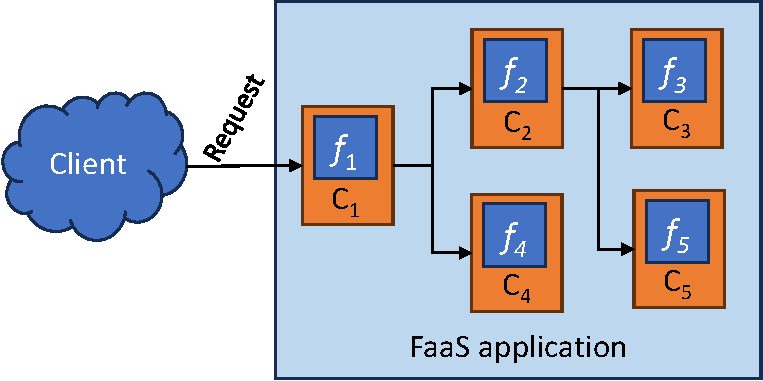
\includegraphics[width=0.8\textwidth]{papers/paper5-cofaas/figures/faas_application.pdf}
\caption{\label{fig:faas-app} A schematic of the execution of a multi-function FaaS application.}
\end{figure}

\section{Instruction Delivery in the Datacenter}
\label{sec:instr-delivery}

% TODO: This was inteded to be a separate sectoin on the BTB but for now it just points here
\label{sec:btb-background}


% Front-end problem -> what people have done
Datacenter workloads are distinguished by having massive
multi-megabyte instruction footprints. These workloads generally have
multi-layered software architectures with deep dependency
stacks. Consider, for example, a server hosting a website. Processing
a request to the website involves invokes the web server, the
interpreter of the backend language powering the website and a
database server. All of these components also involve a large amount
of system calls that perform context switches and execute a
significant amount of kernel
code~\cite{ferdman12_clear_cloud,ailamaki99_dbmss_moder_proces}. These
large code footprints overwhelms the capabilities of current processor
frontends causing a well-documented phenomenon known as the frontend
bottleneck~\cite{kanev15_profil,ferdman12_clear_cloud,ayers19_asmdb,kanev15_profil,kumar17_boomer,kumar18_blast_throug_front_end_bottl_with_shotg,kumar20_shoot_down_server_front_end_bottl,spracklen05_effec_instr_prefet_chip_multip}.


The frontend bottleneck occurs when the frontend of the processor is
unable to deliver a continuous stream of instructions to the backend.
% Write about what happens when the pipeline fills an instruction
Instruction delivery interruptions from the frontend can occur for two
reasons: \begin{inparaenum}[1)] \item the frontend mispredicts the
  next instruction due to a branch misprediction or a branch target
  miss or \item the frontend encounters an instruction cache
  miss.\end{inparaenum}. Recovering from either of these events cause
significant performance deterioration by causing long pipeline stalls
that prevents the processor from making progress for tens of
cycles. When a branch misprediction occurs, the instruction stream
must be resteered onto the right-path execution. Doing this requires a
pipeline flush, exposing the core to a pipeline fill latency of tens
of cycles. L1-I cache misses are even more expensive exposing the core
to the cache fill delay occurring while the right-path instructions are
fetched into the instruction cache.

Traditionally, the instruction cache prefetching capabilities of
processor frontends consisted of only next-line prefetching
(NLP)~\cite{nextline_pref}. In NLP, the next instruction cache block
is prefetched unconditionally. While this technique provide miss
coverage for linear code execution, it is incapable of covering the
discontinuous control flows with large spatial footprints that are
common in server processors. To address this, researchers have
proposed numerous hardware mechanisms for instruction prefetching. We
generally subdivide these into two categories: temporal streaming and
fetch-directed prefetching. We describe these in the following two
sections.

\subsection{Temporal Streaming} Fundamentally, temporal streaming
based prefetching exploit the repetitiveness of program control
flow. The intuition behind this is that even if a program can perform
several operations, the instruction sequence executed to perform a
particular operation is highly repetitive. This principle enables
instruction prefetching through a record and replay
approach. Essentially, this approach records streams of instructions
and subsequently replays them to generate prefetching targets when a
starting instruction is accessed. \textcite{ferdman08_tempor} proposed
Temporal Instruction Fetch Streaming (TIFS), the first prefetcher to
exploit this principle. While TIFS is effective at avoiding
instruction cache misses it requires a massive amount of metadata
storage to save the recorded instruction access streams.  Proactive
Instruction Fetch~\cite{ferdman11_proac_instr_fetch} improves on both
the performance and metadata storage requirements of TIFS by recording
compacted retire-order instruction streams. Still, it requires large
amounts of metadata storage of 200KB per core.  % \truls{Describe other
  % temporal streaming approaches}

To summarize, prefetchers based on temporal streaming are highly
effective at eliminating L1-I misses but they do so at the cost of
requiring large amounts of metadata storage and complex dedicated
logic.

\begin{figure}[ht]
  \centering
  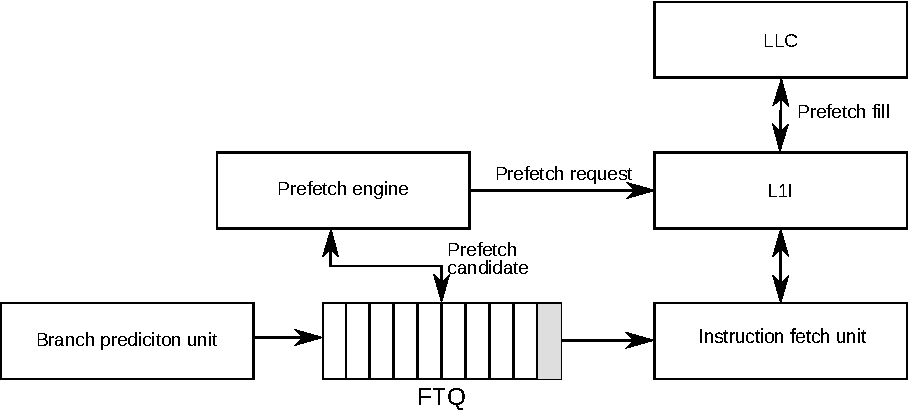
\includegraphics[width=0.8\textwidth]{figures/fdip1.pdf}
  \caption{\label{fig:fdip} A schematic of the FDIP architecture.}
\end{figure}

\subsection{Fetch-directed Prefetching}
The Branch Target Buffer (BTB) has several important roles in a modern high-performance processor \truls{Write more about the BTB}

\textcite{reinman99_fetch_direc_instr_prefet} proposed a prefetching
mechanism known as Fetch-Directed Instruction Prefetching (FDIP). The
key insight of FDIP is that the BTB captures program control flow by
storing branches and their targets. Therefore, it already contains the
metadata needed to identify program control flow divergences and
perform instruction prefetching accordingly. A schematic of FDIP is
shown in \Cref{fig:fdip}. FDIP decouples the branch prediction unit
form the fetch unit using a dedicated queue known as the Fetch Target
Queue (FTQ). This decoupling allows the branch prediction unit to run
ahead of program execution and fill the FTQ with locations of the
future predicted control flow. Thus, the targets in the FTQ are
suitable as instruction cache prefetch candidates since they
correspond to the future control flow of the program being
executed. In spite of FDIP's alluring simplicity and absence of
dedicated metadata storage, conventional wisdom long held that FDIP
wss incapable of effectively covering instruction cache misses in
commercial server workloads. This was considered the case for two
reasons: \begin{inparaenum}[1)] \item Realistically sized BTBs are too
  small to capture the entire branch working set of server
  workloads. This causes frequent BTB misses and the resulting
  frequent pipeline flushes prevents the prefetching from working
  optimally. \item Branch predictor error compounds geometrically with
  the number of branches predicted, \truls{finish}
\end{inparaenum}


\textcite{kumar17_boomer} introduced Boomerang, an instruction
prefetching approach that challenged the conventionally held wisdom
claiming the inadequacy of FDIP prefetchers. Boome\-rang takes a twofold
approach: Firstly, it pre-decodes blocks fetched into the instruction
cache to identify and extract the branches they contain. The extracted
branches are used to pro-actively pre-fill the BTB. Secondly,
Boomerang leverages a basic-block\footnote{A basic-block is defined as
  a sequence of straight-line instructions ending with a branch} based
BTB~\cite{yeh92_compr_instr_fetch_mechan_for}. Since more than one
branch may have targets that lie within the same basic block, this BTB
organization increases the BTB storage density and reduces BTB
misses. Shotgun~\cite{kumar18_blast_throug_front_end_bottl_with_shotg,kumar20_shoot_down_server_front_end_bottl}
improves the miss coverage of Boomerang further by introducing an
optimized BTB organization consisting of three structures. The U-BTB
that stores unconditional branches, the Return Instruction Buffer
(RIB) and the C-BTB that stores conditional branches. The key insight
behind this BTB organization is that unconditional branches tend to
jump far from their origin as they typically represent function calls,
possibly spanning different libraries. Conditional branches, on the
other hand, tend to have targets close to their origin since they
typically represent control flow within a function, such as an
\texttt{if} block or a loop. Furthermore, program control flow often
follow a pattern where a (long) unconditional jump precedes a sequence
of multiple (short) conditional jumps. To effectively track the code
footprints referenced by conditional jumps, each entry of the U-BTB
tracks the spatial footprints of instructions accessed by conditional
jumps around the target and return addresses of the unconditional
jump. When an unconditional branch in the U-BTB is predicted taken,
the code referenced by the associated spatial footprints is prefetched
and the contained conditional branches are decoded and pre-filled into
the C-BTB. The Shotgun BTB organization significantly improves the
storage density and accuracy of the BTB by allowing it to track a
larger portion of the branch working set. This improves the efficiency
and accuracy of FDIP.

These results strongly support the viability of FDIP instruction
prefetchers and disprove conventional wisdom deeming them unsuitable
for covering the massive instruction footprints of server
workloads. This view is supported by a recently presented industrial
perspective from ARM. \textcite{ishii21_re_fetch_direc_instr_prefet}
presents an FDIP prefetching mechanism and argues for its viability in
commercial processors because it requires no additional metadata and
has a minimal implementation complexity overhead. Notably, their
mechanism outperforms the winner of the recent Instruction Prefetching
Championship (IPC-1)~\cite{ipc1}. Based on this, they argue that their
FDIP implementation should be considered the new baseline that
instruction prefetching research proposals are compared
against. Further, they strongly emphasize the importance of ensuring
sufficient BTB capacity in modern processors as FDIP-based prefetchers
are superior from both a performance and implementation perspective
when coupled with a sufficiently large BTB.

\subsection{Serverless Computing and the Front-end Bottleneck}



% \cite{kanev15_profil,ferdman12_clear_cloud}

% \subsubsection{The Branch Target Buffer}

%Two prefetching approaches: FDIP and streaming

% FDIP approaches: \cite{reinman99_fetch_direc_instr_prefet, kumar17_boomer,kumar18_blast_throug_front_end_bottl_with_shotg,kumar20_shoot_down_server_front_end_bottl}

% Streaming approaches:
% \cite{ferdman08_tempor,ferdman11_proac_instr_fetch,kaynak13_shift,kaynak15_confl}

% Profiling based:

% RDIP-based methods are superior but require highly-efficient prefetchers to work. This motivated the development of BTB-X

% Explain diffeernt approaches, prefetching, BTB, cache replacement

% Add a description of the processor frontend


\ifx\chapincluded\undefined
  \printbibliography
  \end{refsection}
 \fi
\end{document}

%%% Local Variables:
%%% mode: latex
%%% TeX-master: t
%%% TeX-command-extra-options: "-shell-escape"
%%% End: